\chapter{Prospects}
\label{sec:prospects}

Obviously, in this script, we were not able to show you the least of what \LaTeX{} has to offer. 
Therefore, in this last section, we gathered some information to help you to go further into depth by yourself.

\section{Packages}

We already have presented a selection of packages. However, there are thousands more of them. In the following sections we have put together some packages for frequently needed features: 

\begin{figure}[p]
	\widebox{
		% Top rules:
		\colrules
		% Left content: code listing:
		\begin{subfigure}{\widefigurewidth}
			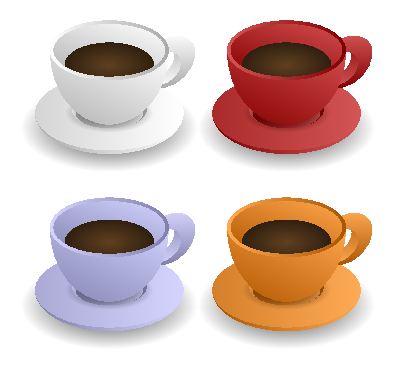
\includegraphics[width=\linewidth]{graphics/coffee-cup.pdf}
		\end{subfigure}
		\hspace{\widefiguregap}
		% Right content: image or rendered example:
		\begin{subfigure}{\widefigurewidth}
			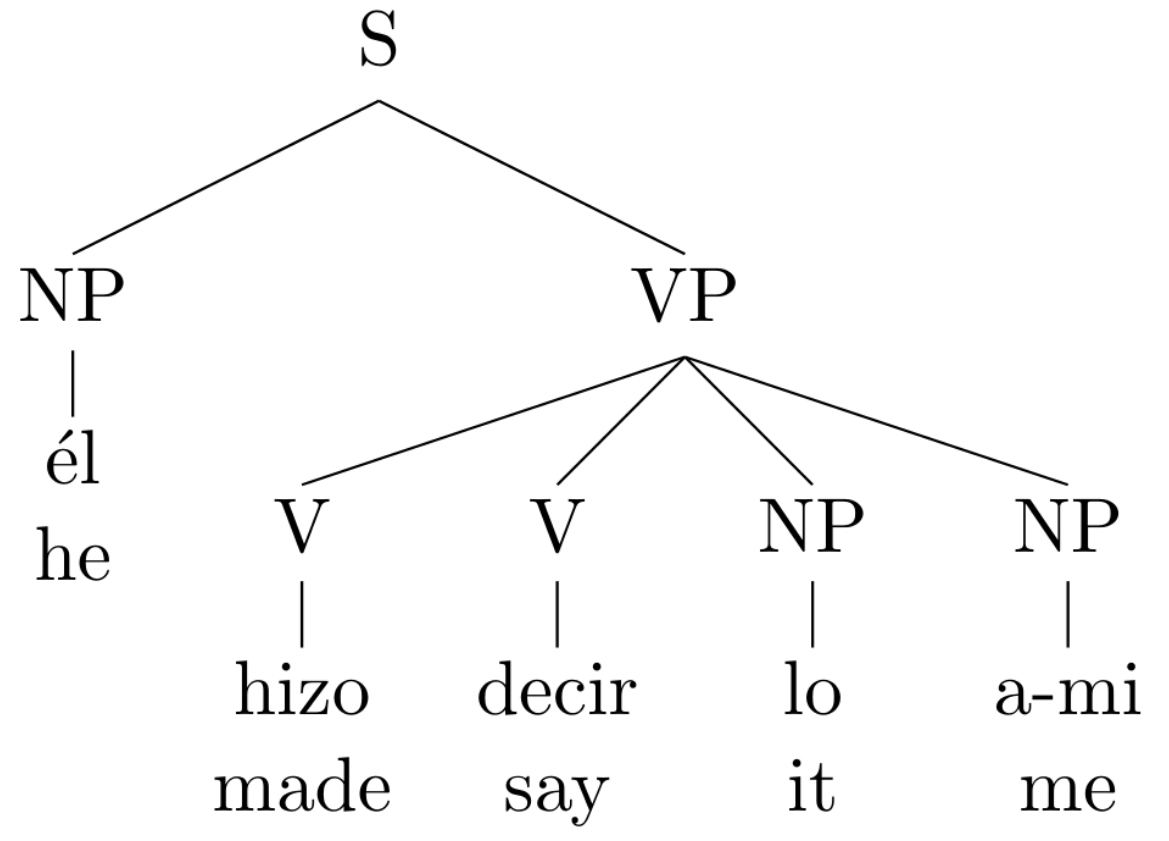
\includegraphics[width=\linewidth]{graphics/qtree.png}
		\end{subfigure}
		% Bottom rules:
		\colrules
		% Left caption:
		\begin{subfigure}[t]{\widefigurewidth}
			\caption{Vector graphics with TikZ}
			\centering\tiny{\url{https://texample.net/tikz/examples/coffee-cup/}}
			\label{fig:tikz-example}
		\end{subfigure}
		\hspace{\widefiguregap}
		% Right caption:
		\begin{subfigure}[t]{\widefigurewidth}
			\caption{Parse trees with qtree}
			\centering\tiny{\url{https://www.ling.upenn.edu/advice/latex/qtree/}}
			\label{fig:qtree-example}
		\end{subfigure}
		\medskip

		% Top rules:
		\colrules
		% Left content: code listing:
		\begin{subfigure}{\widefigurewidth}
			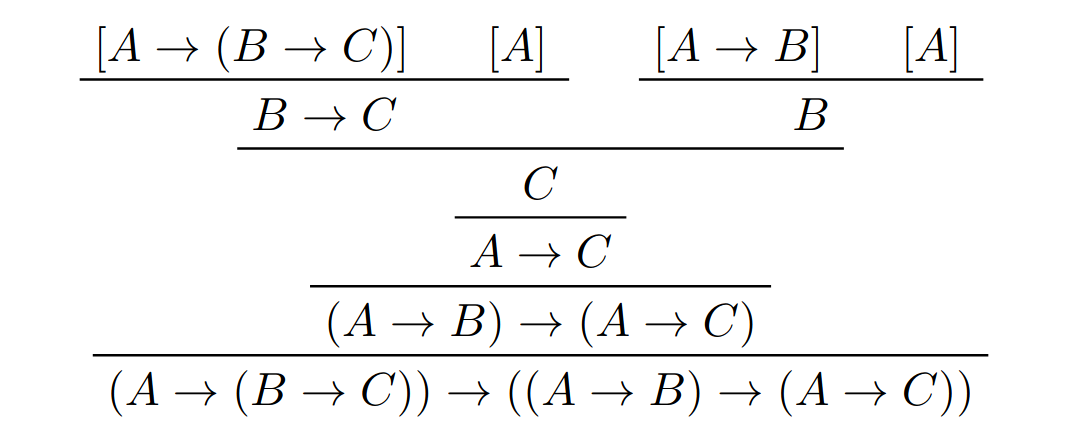
\includegraphics[width=\linewidth]{graphics/prftree.png}
		\end{subfigure}
		\hspace{\widefiguregap}
		% Right content: image or rendered example:
		\begin{subfigure}{\widefigurewidth}
			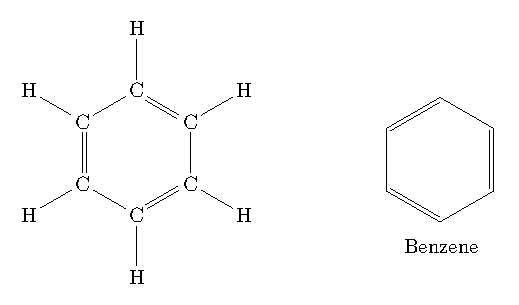
\includegraphics[width=\linewidth]{graphics/benzene-ring.pdf}
		\end{subfigure}
		% Bottom rules:
		\colrules
		% Left caption:
		\begin{subfigure}[t]{\widefigurewidth}
			\caption{Proof trees with prftree}
			\centering\tiny{\url{https://ftp.gwdg.de/pub/ctan/macros/latex/contrib/prftree/}}
			\label{fig:prftree-example}
		\end{subfigure}
		\hspace{\widefiguregap}
		% Right caption:
		\begin{subfigure}[t]{\widefigurewidth}
			\caption{Chemical structural formulas with chemfig}
			\centering\tiny{\url{http://latex-cookbook.net/cookbook/examples/benzene-ring/}}
			\label{fig:chemfig-example}
		\end{subfigure}
		\medskip
	}
	% General caption:
	\caption{Examples for some packages}
	\label{fig:package-examples}
\end{figure}


\begin{description}
	\item[Indices]
		can be created automatically with \texttt{makeidx}.\footnote{\url{https://www.ctan.org/pkg/makeidx}}
		By using \mintinline{tex}{\index{…}}, one can mark entries for the index. With \mintinline{tex}{\printindex}, \replaced[id=C]{an index with references is compiled out of them}{they are assembled within index with references}.
	\item[Vector graphics]
		(\cref{fig:tikz-example})
				can be \enquote{drawn} directly in the \LaTeX{} source code with \texttt{TikZ} (recursive acronym for \emph{TikZ ist kein Zeichenprogramm}, in English: \emph{TikZ is not a drawing program}).\footnote{\url{https://www.ctan.org/pkg/pgf}}
		Caution: This package is very powerful, but not necessarily beginner-friendly.
		Before creating vector graphics from sratch, we recommend you to experiment with some of the examples at \TeX{}ample\footnote{\url{https://texample.net/tikz/examples/}}. 
		\replaced[id=C]{Also, f}{F}or certain use cases, there are special packages that are easier to handle than \enquote{raw} TikZ:
	\item[Parse trees]
		that divide sentences into their grammatical components (\cref{fig:qtree-example}) can be created with \texttt{qtree}.\footnote{\url{https://ctan.org/pkg/qtree}}
	\item[Proof trees,]
		that are often used in logics (\cref{fig:prftree-example}), can be drawn with the package \texttt{prftree}.\footnote{\url{https://www.ctan.org/pkg/prftree}}
	\item[Chemical structural formulas]
		(\cref{fig:chemfig-example})
		can, amongst others, be created with  \texttt{chemfig}.\footnote{\url{https://www.ctan.org/pkg/chemfig}}
	\item[Colors]
		for your documents are provided by \texttt{xcolor}.\footnote{\url{https://www.ctan.org/pkg/xcolor}}
	\item[Note]
		\deleted[id=C]{that you have made in your source code and} that you cannot overlook can be created with \texttt{todonotes}.\footnote{\url{https://www.ctan.org/pkg/todonotes}}
		With the package, \replaced[id=C]{you}{one} can mark what \replaced[id=C]{you}{they} still \todo{Please do not change. This is an example.} have to change within \replaced[id=C]{your}{their} document.
	\item[Pages of other \acro{PDF} files]
		can be integrated into the source code with \texttt{pdfpages}.\footnote{\url{https://www.ctan.org/pkg/pdfpages}}
		It comes in very handy whenever one needs the output of external programs in the document, for example, in\deleted[id=C]{ within} the appendix.
		Just compile the document one more time and the appendix is up-to-date again, if the external program has changed something.
	\item[Nested graphics]
		and the positioning of captions at almost any place are provided by  
		\texttt{subcaption}.\footnote{\url{https://www.ctan.org/pkg/subcaption}}
		We also made extensive use of this package.
	\item[Tables]
		can be designed much more flexibl\replaced[id=C]{y}{e} than what we have shown here. 
		The following packages can help you with that:
		\texttt{colortbl},\footnote{\url{https://www.ctan.org/pkg/colortbl}}
		\texttt{tabularx},\footnote{\url{https://www.ctan.org/pkg/tabularx}}
		\texttt{multirow},\footnote{\url{https://www.ctan.org/pkg/multirow}}
		\texttt{makecell}.\footnote{\url{https://www.ctan.org/pkg/makecell}}
\end{description}

\noindent \texttt{beamer}, which is not a package, but another document class, can be used to create \textbf{slide shows}
with \LaTeX{}. Information on the document class and examples are available at Overleaf,\footnote{\url{https://www.overleaf.com/learn/latex/Beamer}} which brings us to the next section:

\section{Help and information}

\textbf{Wikibooks} provides you with a much more detailed introduction into \LaTeX{}. Note that the German version\footnote{\url{https://de.wikibooks.org/wiki/LaTeX-Kompendium}} is less complete than the English one.\footnote{\url{https://en.wikibooks.org/wiki/LaTeX}}
If required, both refer to additional packages.

Whenever you need information on certain packages, \acro{\textbf{CTAN}}\footnote{\url{https://ctan.org/}} is your place to go. 
\replaced[id=C]{For each package, you can find the official documentation as a \acro{PDF} file there.}{The official documentation as \acro{PDF} for each package can be found there.}
Within this file, the first paragraphs are \added[id=C]{usually }the most interesting. They are 
followed by implementation details, that you normally do not need.

If the official documentation is too theoretical, and you prefer a more hands-on approach, \textbf{Overleaf}\footnote{\url{https://www.overleaf.com/}} can help you out.
Primarily, it is a collaborative online \LaTeX{} editor. However, you can find multiple templates\footnote{\url{https://www.overleaf.com/latex/templates}} for different types of documents (VCs, theses, \textellipsis) there.

If you are looking for examples dedicated to TikZ, \textbf{\TeX{}ample}\footnote{\url{https://texample.net/}} provides you with multiple of them.

For concrete questions, the question-answering platform \textbf{Stackexchange} is a good place to go: There even is a \TeX{} community there.\footnote{\url{https://tex.stackexchange.com/}}

\replaced[id=C]{Of course}{Needless to say}, you can always contact us with your questions:
\begin{compactitem}
	\item via mail to \href{mailto:fachschaft-wiai.stuve@uni-bamberg.de}{fachschaft-wiai.stuve@uni-bamberg.de},
	\item via phone at +49951\,863\,1219,
	\item or just come to our bureau at WE5/02.104.
\end{compactitem}

